\documentclass[letter]{article}
\usepackage{graphicx}
\begin{document}
\DeclareGraphicsExtensions{.png, .jpg, .pdf}

\begin{center}
	\Large\textbf{Tarea 4 Metodos Computacionales}\\
	\large\textit{Julian A. Melendez}
\end{center}
\section{Cuerda Fija}
\begin{figure}[h]
  \centering
    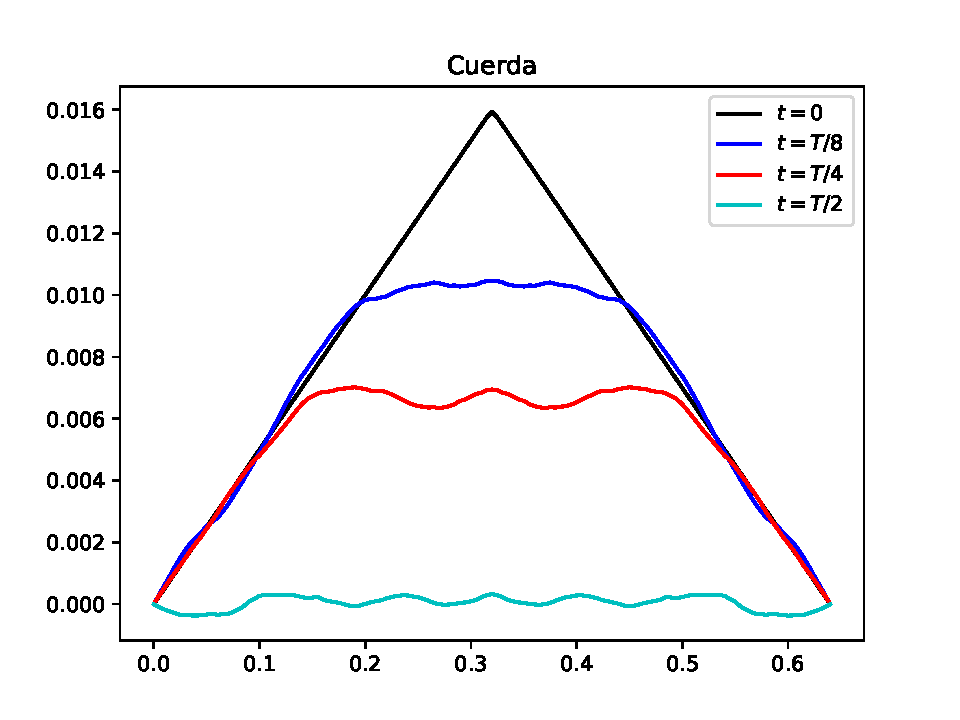
\includegraphics[width=0.9\textwidth]{Cuerda.pdf}
	\caption{Cuerda fija}
\end{figure}
Esta es la solucion de una cuerda con los extremos fijos en 0 sin ninguna perturbacion, la cuerda tiene condicion inicial triangular. 

\newpage
\section{Cuerda con Perturbacion}
\begin{figure}[h]
  \centering
    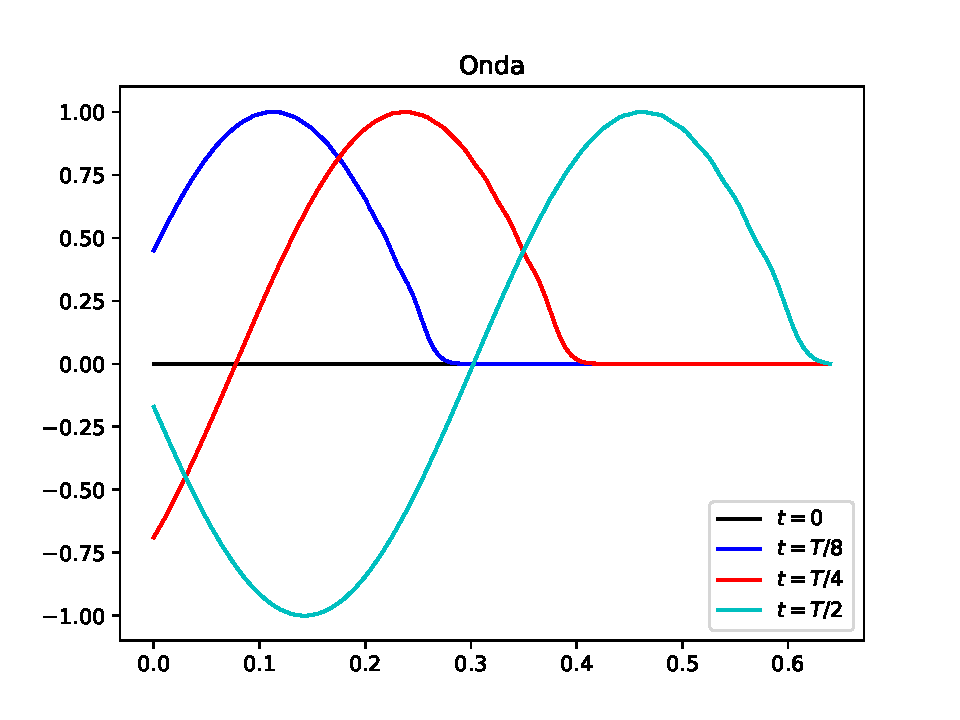
\includegraphics[width=0.9\textwidth]{Onda.pdf}
	\caption{Cuerda con perturbacion}
\end{figure}
Esta es la solucion de una cuerda con los extremos fijos en 0 con perturbacion en un extremo de una funcion seno, la cuerda tiene condicion inicial de amplitud 0. 
\newpage
\section{Membrana de un Tambor}
\begin{figure}[h] 
  \begin{minipage}[b]{0.7\linewidth}
    \centering
    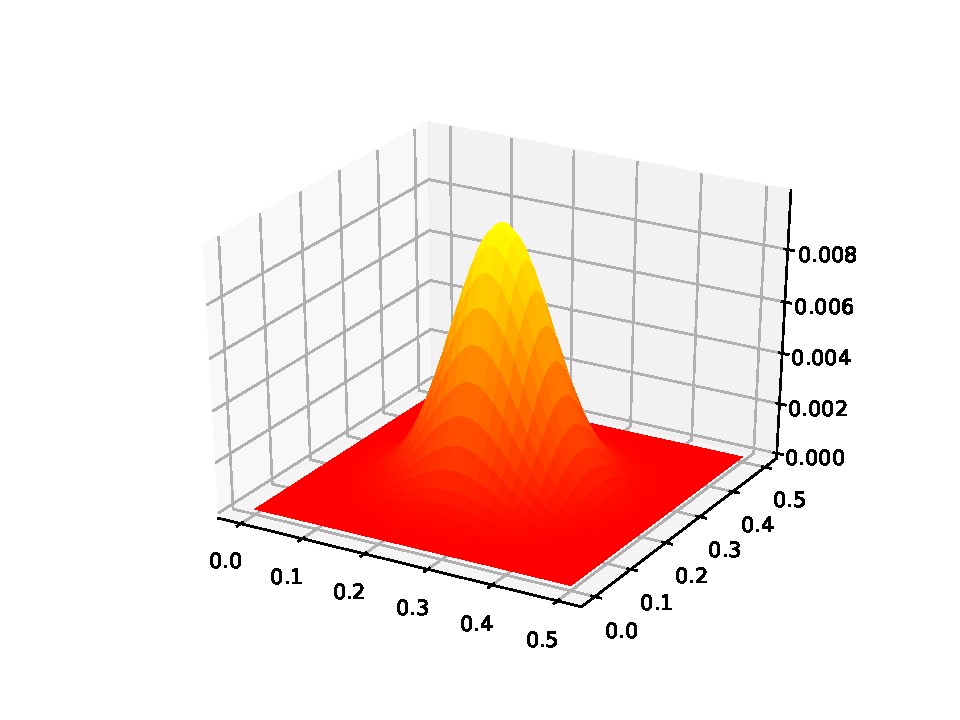
\includegraphics[width=.8\linewidth]{Tambor1.pdf} 
    \caption{Membrana en t=0} 
    \vspace{4ex}
  \end{minipage}%%
  \begin{minipage}[b]{0.7\linewidth}
    \centering
    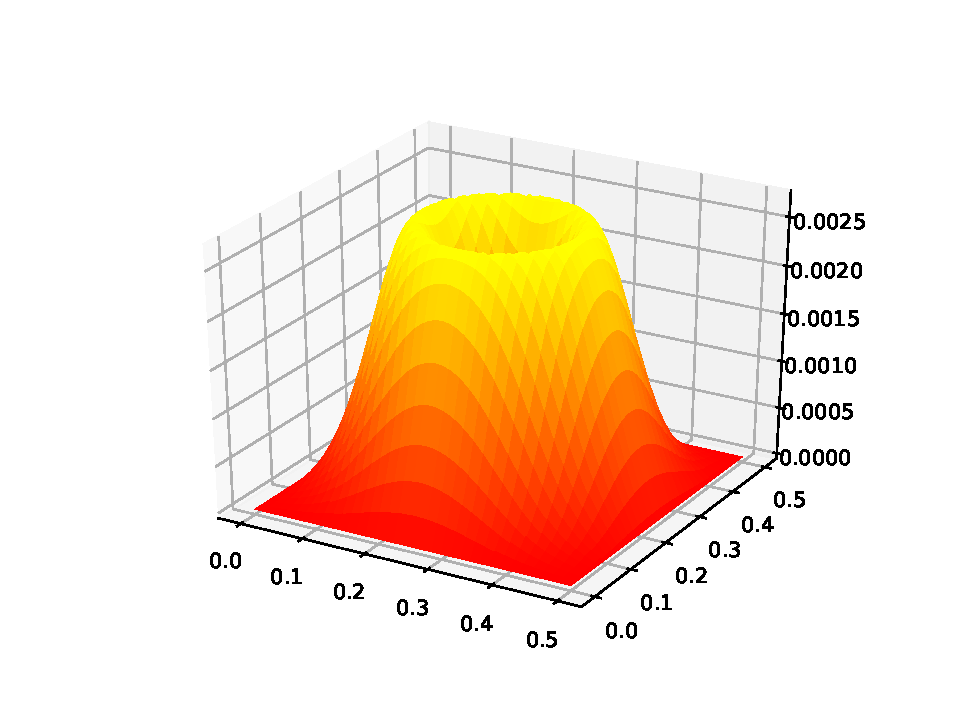
\includegraphics[width=.8\linewidth]{Tambor2.pdf} 
    \caption{Membrana en t=T/8} 
    \vspace{4ex}
  \end{minipage} 
  \begin{minipage}[b]{0.7\linewidth}
    \centering
    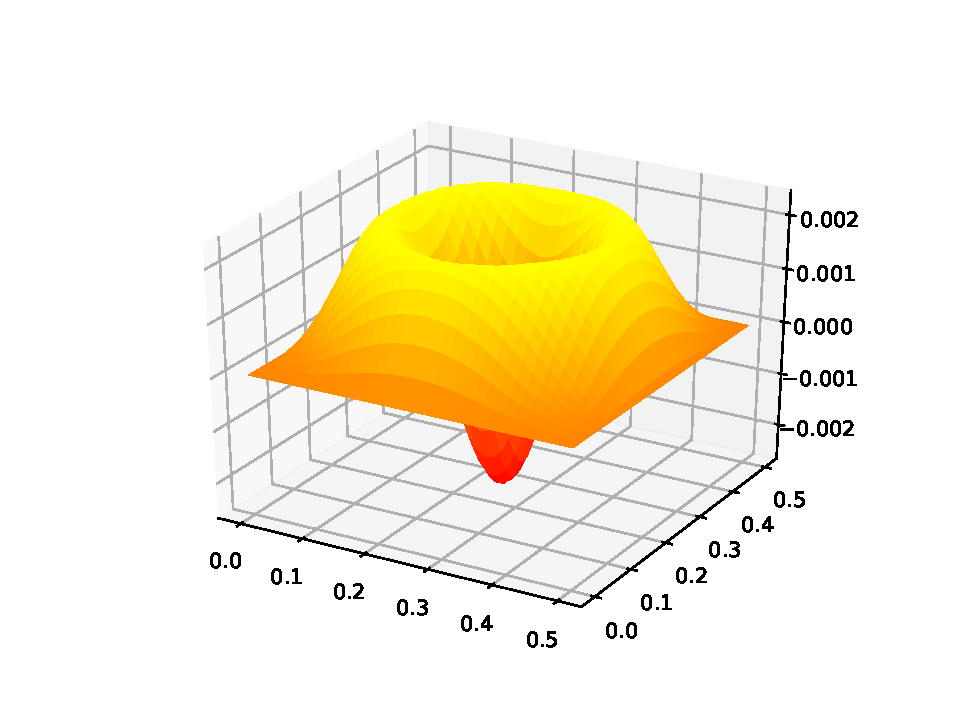
\includegraphics[width=.8\linewidth]{Tambor3.pdf} 
    \caption{Membrana en t=T/4} 
    \vspace{4ex}
  \end{minipage}%% 
  \begin{minipage}[b]{0.7\linewidth}
    \centering
    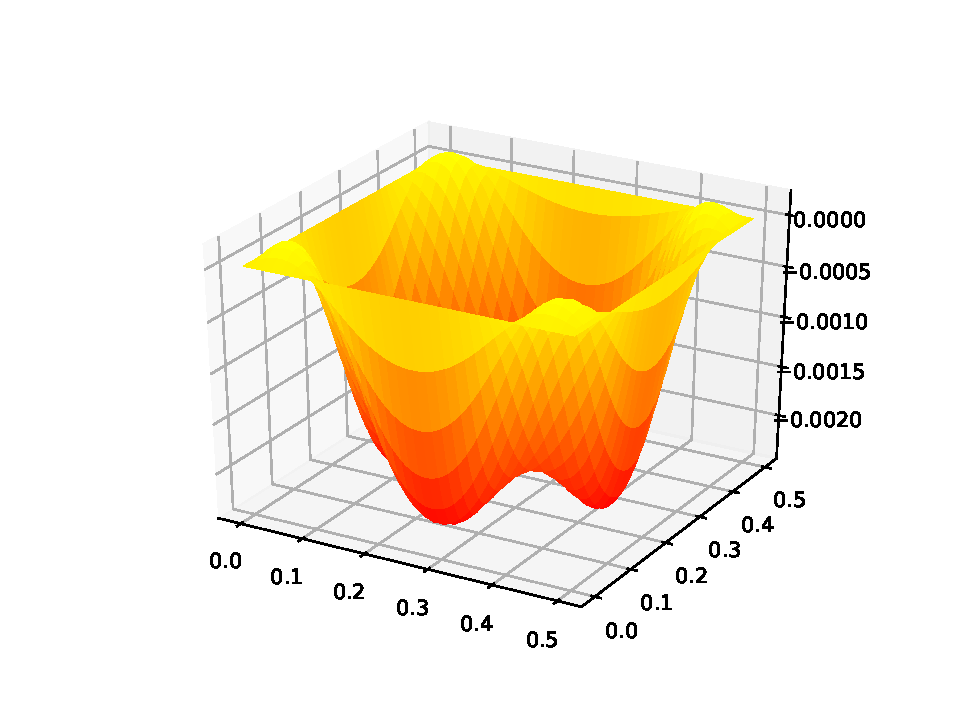
\includegraphics[width=.8\linewidth]{Tambor4.pdf} 
    \caption{Membrana en t=T/2} 
    \vspace{4ex}
  \end{minipage} 
\end{figure}

Las cuatro graficas anteriores muestran la evolucion temporal de la membrana de un tambor al solucionar la ecuacion de onda en dos dimensiones, las graficas son en periodos diferentes.



\end{document}

